\begin{figure}[H]
    \centering
    \begin{tikzpicture}

    % iceberg
    \node at (0,0.8) {
\includegraphics[width=10cm]{images/iceberg.jpg}}; 

    % seuils
    \draw[dashed] (-3.5,2.5) -- (3.5,2.5);
    \draw[dashed] (-3.5,-0.5) -- (3.5,-0.5);
    \draw[dashed] (-3.5,-2) -- (3.5,-2);

    \node at (0,3.2) {\textbf{Maladie à expression clinique}};
    \node at (0,0.8) {\textbf{\gls{mrd}}};
    \node at (0,-1.4) {\textbf{\gls{mrd} non quantifiable}};
    \node at (0,-3) {\textbf{Maladie non détectable}};

    % axe cellules leucémiques 
    \draw[very thick] (-3.5,4.2) -- (-3.5,-4.2);
    \node[rotate=90] at (-4.5,0) {Nombre de cellules leucémiques};

    \node at (-3.9,4.0) {$10^{12}$};
    \node at (-3.9,2.5) {$10^{10}$};
    \node at (-3.9,1) {$10^{8}$};
    \node at (-3.9,-0.5) {$10^{6}$};
    \node at (-3.9,-2) {$10^{4}$};
    \node at (-3.9,-3.5) {$10^{2}$};

    % axe valeurs de mrd
    \draw[very thick] (3.5,4.2) -- (3.5,-4.2);
    \node[rotate=-90] at (4.7,0) {Valeurs de \gls{mrd}};

    \node at (4,2.5) {$10^{-2}$};
    \node at (4,1) {$10^{-4}$};
    \node at (4,-0.5) {$10^{-6}$};
    \node at (4,-2) {$10^{-8}$};
    \node at (4,-3.5) {$10^{-10}$};

    % Techniques de détection
    \node[align=center, text width=4cm, font=\bfseries] at (7,4.4) {Méthodes de mesure};

    \node[anchor=west] at (5.5,3.3) {
\includegraphics[width=1.5cm]{images/microscope.png}};
    \node[anchor=west] at (7.8,3.3) {Microscopie optique};

    \node[anchor=west] at (5.5,1.5) {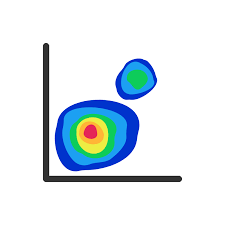
\includegraphics[width=1.5cm]{images/cmf.png}};
    \node[anchor=west] at (7.8,1.5) {\gls{cmf}};

    \node[anchor=west] at (5,0) {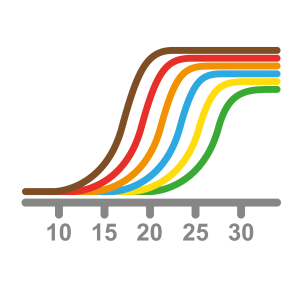
\includegraphics[width=1.5cm]{images/pcr.png}};
    \node[anchor=west] at (7.8,0) {\gls{pcr} quantitative};

    \node[anchor=west] at (6.2,-0.5) {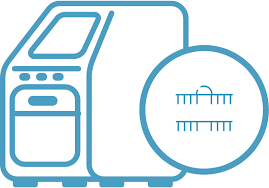
\includegraphics[width=1.5cm]{images/ngs.png}};
    \node[anchor=west] at (7.8,-0.5) {\gls{ngs}};

    \node[align=center] at (7.5,-2.5) {\gls{mrd} non détectable \\ avec les méthodes actuelles};
    \node[align=center] at (7.5,-3.5) {\textbf{Guérison}};

    \end{tikzpicture}
    \caption{
    Représentation schématique des techniques de détection de la \gls{mrd} et des seuils de détection en 
    regard du nombre de cellules leucémiques.
    Les techniques de détection sont classées selon leur sensibilité, allant de la morphologie à la biologie 
    moléculaire. Adapaté de \citeauthor{sayginMeasurableResidualDisease2022} \cite{sayginMeasurableResidualDisease2022}.
    }
    \label{fig:mrd-techniques}
\end{figure}

